\documentclass[aps, prc, reprint, amsmath, groupedaddress, nofootinbib]{revtex4-1}
%\usepackage[compat=1.1.0]{tikz-feynman}
\usepackage[utf8]{inputenc}
\usepackage{hyperref}
\usepackage{amsmath}
\usepackage{amssymb}
\usepackage{amsfonts}
\usepackage{tabularx}
\usepackage{booktabs}
\usepackage{graphicx}
\usepackage{color}
\usepackage{multirow}
\usepackage{verbatim}
\usepackage[inline]{enumitem}
\graphicspath{{fig/}}
\definecolor{theblue}{RGB}{0,50,230}
\usepackage{appendix}
\hypersetup{
  colorlinks=true,
  linkcolor=theblue,
  citecolor=theblue,
  urlcolor=theblue
} 


\begin{abstract}
A Monte-Carlo simulation is a useful tool in the phenomenological study of the jets in the heavy-ion collisions.
However, the medium induced gluon radiation--important at high energy--
is hard to be accurately implemented in a Monte-Carlo way,
because the multiple scatterings cannot be factorized into independent processes due to the coherence effect.
Many existing implementations work in certain limits or capture qualitatively behaviors, but it is important to develop an approach that quantitatively agrees with the current knowledge from theory.
In this work, we discussed the ingredients of three specific implementations and compared them to the perturbative calculation.
The ``Modified rescattering" approach reproduces the semi-analytic calculations of the parton radiative energy loss and reasonably explains the gluon spectra in a static medium.
The impacts of an expanding medium, running coupling and mass effect are also discussed. 
With a controlled modeling uncertainty between the Monte Carlo model and the theory, a more meaningful extraction of the jet transport property in a quark-gluon plasma can be performed in the future.
\end{abstract}

\begin{document}
\title{Calibrating Monte-Carlo implementations of parton radiative energy loss to theoretical calculations}
\author{Weiyao Ke}
\author{Yingru Xu}
\author{Steffen A.\ Bass}
\affiliation{Department of Physics, Duke University, Durham, NC 27708-0305}
\date{\today}
\maketitle 

\section{Introduction}
The study of hard probes in relativistic heavy-ion collisions is moving towards the precision era thanks to the future experimental upgrades \cite{ATLAS-Collaboration:2012iwa,Abelevetal:2014dna,STAR:upgrade-hf,Adare:2015kwa,CMS:2017dec}.
On the phenomenology side, it is imperative to revisit our assumptions and approximations to do a more precise model-to-data comparison to extract interested properties of the quark-gluon plasma (QGP) via hard probes.
Statistical analysis of medium evolution models by comparing to soft-observables have shown success in extracting the temperature dependent shear and bulk viscosity, benefiting from both high accuracy data and models with well controlled uncertainties that allow parameter fine-tuning \cite{Bernhard:2016tnd, Bernhard:2018hnz}.
Applying this analysis to the extraction of jets and heavy quark transport coefficients, we encountered new difficulties. 
First, the transport coefficients have both temperature and momentum dependences, increasing the complexity of uncertainty parametrization \cite{Xu:2017obm}.
Second, the model (theory) uncertainties are large. 
Model uncertainties originate not only from different assumptions that define different theories \cite{CaronHuot:2010bp, Rapp:2018qla} but also from numerical approximations used in practical implementations.
Because model uncertainties obscure the interpretation of the extracted physical quantities, we want to keep them under control.
For the examination of different theory assumptions, such as whether the nature of the interaction is perturbative or non-perturbative or even both, there are ongoing efforts from the JETSCAPE collaboration to interface different theories in a unified way \cite{Cao:2017zih, Kauder:2018cdt}.
In this work, we aim to reduce the uncertainty that comes from the numerical implementations of a specific type of theory, which is the perturbative QCD (pQCD) based transport theory.

The theory of applying pQCD to partonic transport has been developed over the years \cite{Arnold:2002zm, Ghiglieri:2015ala}.
In a near equilibrium medium, energetic partons interact with medium through both elastic (collisional) and inelastic (medium induced gluon radiation) processes at leading order.
Because of the complexity of an evolving and fluctuating medium in realistic collisions, Monte Carlo implementations of the pertubative physics are developed for phenomenology study.
At high energy, the largest uncertainty that is introduced in these Monte Carlo generators comes from different treatments of the gluon radiation since it is the dominant source of energy loss at high energy.
In a dense medium, the QCD Landau-Pomeranchuk-Migdal (LPM) effect is important for such radiations, where multiple scatterings during the gluon formation time act coherently to suppress the radiation spectrum \cite{PhysRev.103.1811,Wang:1994fx,Zakharov:1996fv,Baier:1996kr}.
Therefore, a medium induced radiation becomes effectively an $n$-body to $(n+1)$-body process that extends in space-time.
This feature is particularly difficult to be accurately implemented in a Monte-Carlo way, where interactions are usually built from few-body processes that are local.
To simplify the problem while still keep the essential qualitative features such as the characteristic spectrum and path-length dependent energy loss, different methods are used for numerical simulations \cite{Djordjevic:2008iz,Cao:2013ita,ColemanSmith:2012vr,Xu:2004mz,Zapp:2011ya,Gossiaux:2012cv,Park:thesis}.
In this work we compare quantitatively three implementations with different physical motivations to the knowledge from the perturbative calculations in idealized limits.
Among them, a modified approach based the method of \cite{Zapp:2011ya} works remarkably well.
This method, referred to as the ``Modified rescattering" approach, reproduces the analytic calculations of energy loss as function of coupling constants, temperatures, parton energies and path lengths.
It also reasonably explains the gluon radiation spectrum.
We introduce parameters to control its finite- and infinite-size behaviors separately.
The parameters can be fine-tuned to match the theory or be calibrated to experimental data;
therefore, the performance of the theory can be measured quantitatively on the landscape of this parameter space in future statistical analysis.

This paper is organized as follows. Section \ref{section:qual} reviews the qualitative spectrum of the medium induced radiation.
In Section \ref{section:MC}, three Monte Carlo implementations of the radiative processes are discussed. 
Semi-analytic results to which the Monte Carlo simulations are compared are briefly summarized in Section \ref{section:Theo}.
The major results are discussed in Section \ref{section:results}.
Finally, we discuss in Section \ref{section:disscuss} the running coupling effect, expanding medium effect and the mass (dead-cone) effect in the ``Modified rescattering" implementation. We summarize in Section \ref{section:summary}.

\section{Qualitative features of the medium induced radiation}\label{section:qual}
In this section, we introduce the qualitative features of the medium induced radiation following the discussion in \cite{Baier:1996kr}.
A radiated gluon stays in coherence with the mother partons for a finite amount of time determined by the uncertainty principle $\Delta t \sim 1/\Delta E$. 
$\Delta E$ is the difference in light-cone energy between the initial mother patron energy $E$ and the final state of daughter partons.
The formation time is then,
\begin{eqnarray}\label{eq:tau_1}
\tau_f \sim \frac{2(1-x)\omega}{k_\perp^2+(1-x)m_g^2}.
\end{eqnarray}
$x = \omega/E$ is the energy fraction carried by the gluon. 
$m_g^2$ is the gluon thermal mass squared is related to the Debye screening mass by $m_g^2 = m_D^2/2 \sim \alpha_s T^2$.
For a collinear splitting, the formation time looks like $\omega/(\alpha_s T^2)$ .
Meanwhile, the gluon can keep interacting with the dense medium via elastic collisions with a rate $R_{g}$ that scales like $\alpha_s T$. 
Therefore, the number of rescatterings within the formation time $N \sim \tau_f R_g \sim \omega/T$ may not be a small number for gluon with energy comparable or larger than the medium temperature.
Because rescatterings also change the transverse momentum $k_\perp$ of the gluon relative to the mother parton, a self-consistent formation time estimation is required.
Given that on average elastic scattering increases $k_\perp^2$ by an amount $\hat{q}_g\tau_f$ where $\hat{q}_g = d\langle k_\perp^2\rangle/dt$ is the gluon transport coefficient, the self-consistent relation for an averaged formation time is,
\begin{eqnarray}\label{eq:tau_n}
\tau_f \sim \frac{2(1-x)\omega}{\hat{q}_g\tau_f} \longrightarrow \tau_f \sim \sqrt{\frac{2(1-x)\omega}{\hat{q}_g}}
\end{eqnarray}
The inverse of the formation time measures the rate of a gluon being separated from the mother parton.

The radiation spectrum is understood as follows. 
A virtual gluon with energy $\omega$ and transverse momentum $k_\perp$ splits from the mother parton with the probability given by the vacuum splitting function ($P(x) \sim \alpha_s/x$).
If its formation time is smaller than the mean-free-path of elastic scattering $\lambda_g = 1/R_g$, it is put on shell with the rate $1/\lambda_g$ (the Bethe-Heitler region); otherwise multiple rescatterings put it on-shell with a rate $1/\tau_f$ (the LPM region).
As a result, the differential radiation rate is,
\begin{eqnarray}\label{eq:LPM}
\frac{dP}{dt d\omega} \sim \begin{cases}
 \frac{\alpha_s}{\omega} \frac{1}{\lambda_g} \sim \alpha_s^2  \frac{T}{\omega}, \hfill \tau_f \lesssim \lambda_g\\
 \frac{\alpha_s}{\omega} \frac{1}{\tau_f}\sim \alpha_s \sqrt{\hat{q}_g/T^3} \left(\frac{T}{\omega}\right)^{3/2}, \hfill \lambda_g \lesssim \tau_f
\end{cases}
\end{eqnarray}
We note first that in the leading order picture, the LPM effect modifies the single gluon emission rate. 
It does not introduce correlations between subsequent emissions which are higher order effects \cite{Arnold:2016jnq}.
Second, the emission rate at a certain time receives coherent contributions from the collision centers whose locations extend about $\tau_f$ along the path of the mother parton.
Therefore, if the number of scattering centers in a thin medium of size $\lambda_g < L< \tau_{f,\textrm{max}} \sim \sqrt{E/\hat{q}_g}$ are limited, the second line of Equation \ref{eq:LPM} is replaced by,
\begin{eqnarray}
\frac{dP}{dt d\omega} \sim 
 \frac{\alpha_s}{\omega} \frac{1}{\min\{\tau_f,L\}}, \hfill \lambda_g < \tau_f
\end{eqnarray}
The radiative energy loss is obtained by integrating over the differential rate times the gluon energy. 
For the case of an infinite medium, this is
\begin{eqnarray}\label{eq:dE-Linf}
\Delta E/\Delta L \sim \alpha_s^2 \sqrt{ET^3}
\end{eqnarray}
Therefore for high energy patrons, the amount of energy loss is significantly reduced compared to the incoherent calculation $\Delta E/\Delta L \sim \alpha_s^2 E T$.
For a thin medium, the LPM effect leads to the non-linear path length $L$ dependence of the energy loss
\begin{eqnarray}\label{eq:dE-Lfinite}
\Delta E \sim \alpha_s \hat{q} L^2
\end{eqnarray}
When the path length exceeds the $\tau_{f,\textrm{max}}$, $\Delta E$ should smoothly transit to the behavior given by Equation \ref{eq:dE-Linf}.

\section{Different Monte-Carlo implementations}\label{section:MC}
Despite there have been many practices of implementing the LPM physics,
we compared only those approaches that treat this effect non-locally thus result in a path length dependent spectrum.
The framework we worked in is the {\tt Lido} model \cite{Ke:2018tsh}. 
It is originally designed for heavy quark transport inside a QGP. 
In this section, we turn off all quark mass effects (phase-space, matrix-elements) to study light quark first.
The {\tt Lido} model is based on elementary ($2\rightarrow2$) elastic and inelastic pQCD scatterings. 
The inelastic processes include both gluon radiation ($2\rightarrow 3$) and gluon absorption ($3\rightarrow 2$) processes using an improved Gunion-Bertsch approximated matrix-element \cite{Fochler:2013epa,Uphoff:2014hza}.
For the comparison to theory calculations, we only turn on the $2\rightarrow 3$ channel for the high energy quark and the $t$-channel in the elastic scatterings.
Next, we introduce three different LPM effect implementations in detail.

\paragraph*{``Coherence factor" approach} This first approach is the old one used in the {\tt Lido} model. 
It is simular to the higher-twist formula used in the radiation improved Langevin equation \cite{Cao:2013ita} and the Linearized-Boltzmann-Transport-Model \cite{Cao:2016gvr,Cao:2017hhk}.
In the {\tt Lido} model, we start from the incoherent rate of a $2\rightarrow 3$ process using Gunion-Bertsch cross-section $\sigma_\textrm{GB}$,
\begin{eqnarray}\label{eq:GB-rate}
\Gamma = \frac{1}{2E_1}\int\frac{f_i(p_2)d\vec{p_2}^3}{(2\pi)^3 2p_2}2\hat{s}\int d\hat{t}\frac{d\vec{k}^3}{(2\pi)^3 2k}\frac{d\sigma_{\textrm{GB}}}{d\hat{t}d\vec{k}^3}
\end{eqnarray}
The ``Coherence factor" approach implements LPM suppression by multiplying a time-dependent coherence factor to the final state gluon phase space integration in Equation \ref{eq:GB-rate},
\begin{eqnarray}\label{eq:GB-rate-LPM}
\frac{d\vec{k}^3}{(2\pi)^3 2k} \rightarrow \frac{d\vec{k}^3}{(2\pi)^3 2k} 2\left[1-\cos\left(\frac{t-t_0}{\tau_f}\right)\right]
\end{eqnarray}
The modified rate dependents on the time separation $\Delta t = t-t_0$ which is the time elapse from the last gluon emission.
If one makes a small angle scattering approximation to the Gunion-Bertsch matrix-element (please refer to Appendix \ref{app:consistency} for details), the Gunion-Bertsch rate can be rewritten into a diffusion induced radiation rate
\begin{eqnarray}\label{eq:GB-small-angle-rate}
\Gamma = \hat{q}_g\int\frac{\alpha_s}{2\pi}\frac{2C_F dx}{x} \frac{dk_\perp^2}{k_\perp^4}.
\end{eqnarray}
This would be the same as the one used in \cite{Cao:2013ita} if the coherence factor is included.
Either way, the value of $\Delta t$ is only determined at run-time,
but we can still estimate its order-of-magnitude from the following condition:
\begin{eqnarray}\label{eq:delta-t-1}
\nonumber
1 &\sim& \int_0^{\Delta t}\Gamma(t) dt,\\
&=& \Delta t \int d\Gamma \left[1-\frac{\sin(\Delta t/\tau_f)}{\Delta t/\tau_f}\right]
\end{eqnarray}
which means that the probability to have one radiation within $\Delta t$ should be of order $1$ required by the definition of $\Delta t$.
A dimensional analysis (Appendix \ref{app:consistency}) shows $\Delta t \sim 1/\alpha_s T$
We see that this prescription indeed suppresses the spectrum when the formation time is much greater than the mean-free-path. 
However, multiple scatterings are not included since gluons are always produced in $2\rightarrow3$ processes.
Moreover, it introduces correlation between the locations of vertices of subsequent emissions;
especially, no matter how soft the previous radiation is, it affects the next radiation in the same way and the prediction dependents on the minimum gluon energy cut-off in a logarithmic way.

The next two approaches both include multiple-scattering in the foramtion time determiantion with the method motivated by \cite{Zapp:2011ya}.
A gluon is first sampled from a $2\rightarrow3$ inelastic scattering at time $t=t_0$, but it is not immediately regarded as ``formed". 
This gluon may keep interacting with the medium via elastic processes. Both change the gluon transverse momentum $k_{\perp,n}$ and formation time $\tau_{f,n}$ will be changed after each rescattering.
Here, the subscripts $n$ denote the quantities calculated after the $n$-th rescattering.
This continues until the time elapse since $t_0$ just exceeds the gluon formation time after the $n$-th rescattering,
\begin{eqnarray}\label{eq:self-consisten-condition}
\tau_{f, n} < t-t_0 < \tau_{f, n-1}.
\end{eqnarray}
After this amount of time, the gluon is considered to have lost coherence with the mother parton.
The formation time determined in this way fulfills the self-consistent condition of Equation \ref{eq:tau_n}, but it is still tricky to introduce the correct suppression, so we compared the following two approaches. 

\paragraph*{``Block radiation" approach}
An attempt to introduce suppression is by requiring that no other radiation is allowed within $t-t_0$ showed in Equation \ref{eq:self-consisten-condition}, referred to as the ``Block radiation" approach in this paper.
It certainly suppresses the radiation rate and also results in a non-linear path length dependence of the energy loss; however, a closer examination reveals its problems.
First of all, it again introduces correlations between subsequent emission vertices.
But the biggest problem is that it does not alter the spectrum shape, because though each branching is delayed by $\tau_f$, it is still generated according to the incoherent differential probability. 
The $2\rightarrow 3$ spectrum is only suppressed by an overall factor $1/N$ that reduces $N$ possible inelastic collisions to a single one,
\begin{eqnarray}
N \sim \frac{\left\langle\tau_{f,N}\right\rangle}{ \lambda_{\textrm{inel}}}.
\end{eqnarray}
This is also different from the expected qualitative behavior: it is  $\lambda_{\textrm{el}}$ instead of $\lambda_{\textrm{inel}}$ that should be used.
This approach is certainly not working, but we keep it as an example to show what not to do.

\paragraph*{``Modified rescattering" approach} Finally, we implement an elaborate approach that is modified from the one studied in \cite{Zapp:2011ya,Park:thesis,Park:2016jap}.
We first introduce a few concepts before going to the steps of implementation.

Comparing to previous works, we define an ``effective" mean-free-path $\tilde{\lambda}$,
\begin{eqnarray}\label{eq:effmpf}
\tilde{\lambda} = \frac{m_D^2}{\hat{q}_g(\omega, T)}
\end{eqnarray}
Unlike the mean-free-path that may be sensitive to the regulator, it only relates to well defined quantities and also applies to models with diffusion approximation of elastic processes so long as $\hat{q}$ is given.
We benefit from this feature and implement a general case where large-angle ($|\hat{t}| > h m_D^2$) elastic scatterings are solved by a rate equation while small-angle ($|\hat{t}| < h m_D^2$) processes are solved by a diffusion equation with $\hat{q}_g(|\hat{t}|<h m_D^2)$.
Similarly, the inelastic processes are also separated into a large-angle triggered $2\rightarrow 3$ scattering (Equation \ref{eq:GB-rate} with $|\hat{t}| > h m_D^2$) and a small-angle diffusion induced radiation part {Equation \ref{eq:GB-small-angle-rate} with $\hat{q}_g(|\hat{t}|<h m_D^2)$.  
Though this separation is shown to be equavalent to the leading order transport equation \cite{Ghiglieri:2015ala}, it improves the model in the following ways.
First, the model is not plagued by a rate that diverges when $\hat{t} \rightarrow 0$.
Second, a tuning of $h$ interpolates the model between the diffusion picture and the scattering picture. 
Third, one can employ parametric form instead of the leading order calculation of $\hat{q}_g(|\hat{t}|<hm_D)$ to extract parameters from a model-to-data comparison.

Another change is the redefinition of the gluon formation time off a quark,
\begin{eqnarray}\label{eq:formation-time-def}
\tau_f = \frac{2(1-x)\omega}{\left(1-x+C_F/C_A x^2\right)k_\perp^2 + (1-x)m_g^2}.
\end{eqnarray}
The additional factor in front of $k_\perp^2$ is motivated by the theory to be discussed in the next Section.
It means that the system under consideration is not a only a gluon but a system consists of both the mother quark and daughter partons. 
This factor goes back to one in the soft limit $x\ll 1$, but it increases the formation time for harder splitting. 

With these building blocks, we present the following step-by-step implementation,
\begin{itemize}
\item[1.] Within $\Delta t$, a mother parton undergoes both large-angle inelastic scattering and diffusion induced radiation with rates from Equations \ref{eq:GB-rate} and \ref{eq:GB-small-angle-rate}.
\item[2.] If a gluon $i$ is sampled at $t_{i,0}$, it is appended to a ``pre-gluons" list associated to the mother parton. But its energy is not carried away from the mother.
\item[3.] Loop over the ``pre-gluons" list. 
\begin{itemize}
\item[3.1] If $\tau_f > t-t_{i,0}$, evolve this gluon by both large-angle elastic scatterings and small-angle diffusion. Recalculate its formation time.
\item[3.2] If $\tau_f < t-t_{i,0}$, accept it with probability $p = \min\{1, u\tilde{\lambda}/\tau_f\}$. Accepted gluons are formed and their energies are subtracted from the mother. Otherwise, they are removed from the list without causing energy loss.
\end{itemize} 
\item[4.] Repeat for the next time step.
\end{itemize}
Here, we use the term ``pre-gluons" to denote those gluons that stays in coherence with the mother parton.
A parton may carry an arbitrary number of ``pre-gluons" and there are no correlations among them.
The formation time calculated after multiple scatterings scales like $\sqrt{\omega/\hat{q}}$ on average, so the factor $\tilde{\lambda}/\tau_f$ guarantees that the radiation spectra in the LPM region scales like the qualitative one in Equation \ref{eq:LPM}.
Now we explain the meaning of the other factor $u$.
We first point out that the formation time from the above procedure is only valid to leading-log level.
In the Monte-Carlo simulation, the final transverse momenta $k_\perp^2\sim \tau_f \hat{q} \sim \tau_f \alpha_s^2 T^3 \ln(Q_0^2/m_D^2)$, 
and $Q_0^2\sim \hat{s}$ is the maximum momentum transfer squared in each elastic scattering.
However, from a total coherent point of view, these re-scatterings acts like a single one except that the maximum $Q_0^2$ should be of the order of $k_\perp^2 = \tau_f \hat{q}$.
Therefore, there is a mismatch in the argument of the logarithm.
The $u$ term is introduced to correct for this mismatch,
\begin{eqnarray}
u &=& \left\{\frac{\ln\left(1+\frac{\tau_f\hat{q}}{m_D^2}\right)}{\ln\left(1+\frac{\hat{s}}{m_D^2}\right)}\right\}^{\frac{1}{2}}
\approx \left\{\frac{\ln\left(1+\tau_f/\tilde{\lambda}\right)}{\ln\left(1+\frac{6\omega T}{m_D^2}\right)}\right\}^{\frac{1}{2}}
\end{eqnarray} 
where we have used $\left\langle\hat{s}\right\rangle \approx 6 \omega T$.
This is also motivated by the next-to-lead-log approximation of AMY equation quoted in the next section.

Finally, we point out that Equations \ref{eq:effmpf} and \ref{eq:formation-time-def} only encodes the scaling of these quantities, so in practice we introduce the following tunable relations,
\begin{eqnarray}\label{eq:tune}
\nonumber
\tau_f & \rightarrow & C_1 \tau_f, \\
\tilde{\lambda} & \rightarrow & C_2 \tilde{\lambda}.
\end{eqnarray}
The parameters $C_1$ and $C_2$ are ones by default and controls the finite- and infinite-size behaviors. 
This is possible by realizing that the comparison between medium length and the formation time solely determines the finite size effect; while the acceptance alone controls the magnitude of suppression.
Though it is possible to fine-tuning these parameters systematically, we will show that the default $C_1 = 1, C_2 = 1$ already works very well.

%These parameters are also handles to deform the simulations away from the underlying theory in a controllable way.
%Their values fine-tuned to experiments are not necessarily the same as those tuned to theory. 
%The parameter space $(C_1, C_2)$ can be the map showing the distance from the theory to the phenomenology model required by data.

%Finally, we point out that those ``pre-gluons" in this approach do not have to be medium induced from the very beginning. 
%Gluons from the vaccum shower of a hard parton generated by, {\tt Pythia} e.g., can also be initialized as ``pre-gluons" associated to the hard parton to study the interplay between the vacuum shower and the medium effect.
%Of course this is already out of the scope of the current paper.

\section{Semi-analytic formula for radiative energy loss}\label{section:Theo}
The main purpose of this study is to gauge Monte Carlo implementations using theory.
The full lead-order calculation and the comparison between different approximations have been discussed in detail in \cite{CaronHuot:2008uh}.
The full calculation is quite involved and has to be solved numerically, we only quote its results in the study of finite-size radiation spectra.
For other comparisons, we make use of two (semi-)analytic results where medium induced gluon radiation is solved in an infinitely large medium (to next-to-leading-log accuracy) and in a thin medium (to leading-log accuracy).
For readers convenience, we briefly summarize their formula in this section.

\begin{figure*}
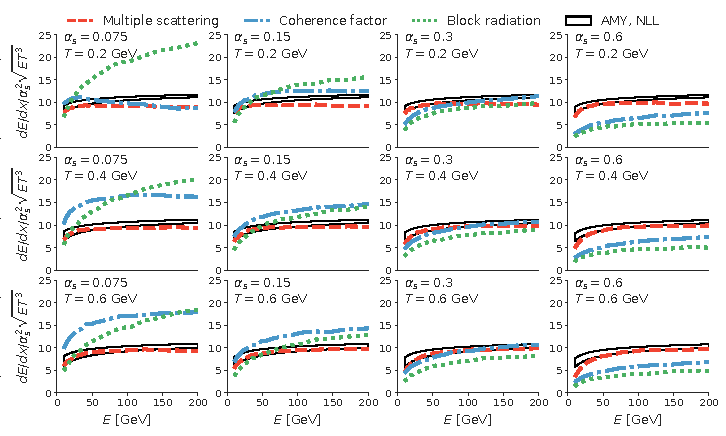
\includegraphics[width=\textwidth]{Eloss_infinite.pdf}
\caption{Energy loss per unit path lengh $dE/dx$ as a function of energy $E$, temperature $T$ and coupling constant $\alpha_s$. Each column corresponds to $\alpha_s = 0.075, 0.15, 0.3$, and $0.6$ (from left to right). Each row corresponds to $T = 0.2, 0.4$, and $0.6$ GeV (from top to bottom). $dE/dx$ is divided by the expected scaling $\alpha_s^2 \sqrt{ET^3}$. The calculations from ``Modified rescattering", ``Coherence factor", and ``Block radiation" approaches are the red-dashed lines, blue-dash-dotted lines, and green-dotted lines respectively. The AMY NLL results are denoted as black boxes.}
\label{fig:eloss-inf}
\end{figure*}

\begin{figure*}
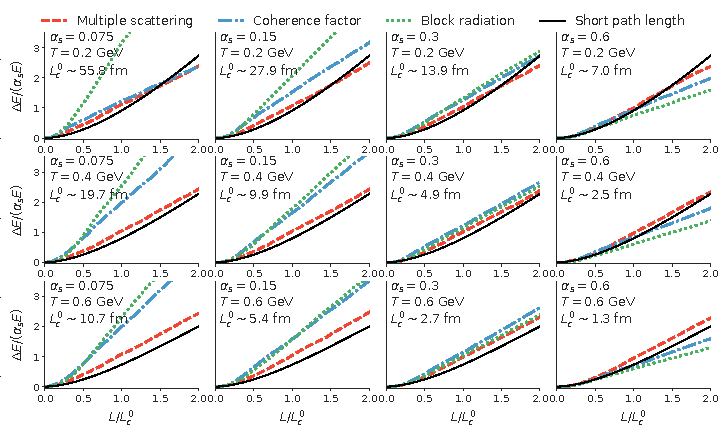
\includegraphics[width=\textwidth]{Eloss_Ldep.pdf}
\caption{Energy loss $\Delta E$ as a function of path length $L$, temperature $T$ and coupling constant $\alpha_s$. Each column corresponds to $\alpha_s = 0.075, 0.15, 0.3$, and $0.6$ (from left to right). Each row corresponds to $T = 0.2, 0.4$, and $0.6$ GeV (from top to bottom). $\Delta E$ is scaled by $\alpha_s E$ and $L$ is scaled by an estimated critical path length $L_c^0 = \sqrt{E/\hat{q}_0}$, $\hat{q}_0 = C_A \alpha_s T m_D^2$. The calculations from ``Modified rescattering", ``Coherence factor", and ``Block radiation" approaches are the red-dashed lines, blue-dash-dotted lines, and green-dotted lines respectively. The analytic results for thin medium are denoted as black solid lines.}
\label{fig:eloss-ldep}
\end{figure*}

\begin{figure}
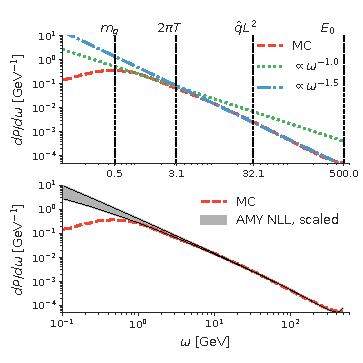
\includegraphics[width=\columnwidth]{spectrum.pdf}
\caption{Radiated gluon spectrum in an infinite medium from a quark $E=500$ GeV, $\alpha_s = 0.1$. The top plot shows the spectrum (red-dashed line) and power law fit (green-dotted and blue-dash-dotted lines) in different gluon energy ($0<\omega < E$) regions, separated by energy scale $m_g$, $\hat{q}_0\lambda_g^2 \sim 2\pi T$. The middle plot is the same simulation compared to the incoherent spectrum and the AMY semi-analytic result. The bottom plot is the ratio between the Monte-Carlo simulation and the semi-analytic calculation.}
\label{fig:spectrum}
\end{figure}

\begin{figure}
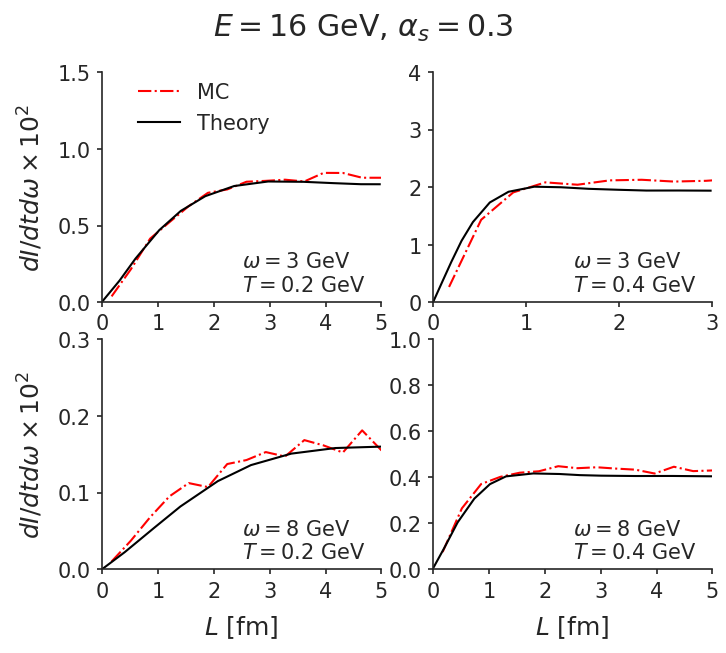
\includegraphics[width=\columnwidth]{spectrum_L.pdf}
\caption{Compare the path-length dependent energy-differential rate $dP/(dtd\omega)$ from Monte-Carlo simulation using $\alpha_s = 0.3$ to the theoretical calculation \cite{CaronHuot:2008uh}. The light quark energy is $16$ GeV. For each $\omega$, the gluon energy within $\omega \pm 0.5$ GeV are used to compute the differential rate.}
\label{fig:spectra-L-alphas=0.3}
\end{figure}

In an infinite static medium, the formula for gluon radiation spectrum (we only use the one for gluon splitting from a quark) is derived in \cite{Arnold:2002zm,Arnold:2003zc},
\begin{eqnarray}\label{eq:AMY-1}
\nonumber
\frac{dP_{q\rightarrow qg}}{dt dx} &=& \frac{1}{2E\nu_q} \frac{\alpha_s d_F P_{q\rightarrow qg}(x)}{2x^2(1-x)^2}\int\frac{d^2\vec{h}}{(2\pi)^2}2\vec{h}\cdot \mathfrak{Re} \vec{F} \\
&\times& [1+f_g(xp)][1-f_q((1-x)p)],
\end{eqnarray}
where $\vec{F}(\vec{h}; p, x)$ satisfies the following equation,
\begin{eqnarray}\label{eq:AMY-2}
\nonumber
2\vec{h} &=& i\frac{h^2 \vec{F}(\vec{h})}{p^3 2x(1-x)} \\
\nonumber
&+& g^2\int \frac{dq_\perp^2 \mathcal{A}(q_\perp^2)}{(2\pi)^2}\left\{\frac{C_A}{2}\left[\vec{F}(\vec{h}) - \vec{F}(\vec{h}+p\vec{q}_\perp)\right]\right. \\
\nonumber
&& \phantom{} + \left(C_F - \frac{C_A}{2}\right)\left[\vec{F}(\vec{h}) - \vec{F}(\vec{h}-xp\vec{q}_\perp)\right] \\
&& \phantom{sss} + \left. \frac{C_A}{2}\left[\vec{F}(\vec{h}) - \vec{F}(\vec{h}-(1-x)p\vec{q}_\perp)\right] \right\}.
\end{eqnarray}
The collision kernel of a gluon in a thermalized QGP is,
\begin{eqnarray}
\mathcal{A}(q_\perp^2) = \frac{T m_D^2}{q_\perp^2(q_\perp^2+m_D^2)}.
\end{eqnarray}
The exact solution can be obtained numerically, but the author of \cite{Arnold:2008zu} obtained a semi-analytic solution to the next-to-leading-log ($[\ln(E/T)]^{-1}$) accuracy that is easier to use,
\begin{eqnarray}\label{eq:AMY-NLL}
\frac{dP_{q\rightarrow qg}^{\textrm{NLL}}}{dt dx} &=& \frac{\alpha_s P_{q\rightarrow qg}(x)}{2\pi}\frac{ \sqrt{2} d_F }{\nu_q }  \frac{m_D^2\hat{\mu}_\perp^2(x)}{2x(1-x)E}. 
\end{eqnarray}
Because we do not use quantum statistics in the Monte Carlo simulations, we have dropped the Bose enhancement and the Pauli blocking factors compared to the original formula.
The remaining terms are organized so that the last factor plays the role of the inverse formation time.
The dimensionless quantity $\hat{\mu}_\perp^2(x)$ is determined by the self-consistent condition,
\begin{eqnarray}\label{eq:AMY-sf}
\nonumber
\hat{\mu}_\perp^2 && = \frac{gT}{m_D} \sqrt{\frac{2x(1-x)E}{\pi T}}\left\{
\frac{C_A}{2}(1-x)^2\ln\left[\frac{\xi\hat{\mu}_\perp^2}{(1-x)^2}\right] + \right. \\
&&\left.\left(C_F-\frac{C_A}{2}\right)x^2\ln\left(\frac{\xi\hat{\mu}_\perp^2}{x^2}\right) + \frac{C_A}{2}\ln(\xi\hat{\mu}_\perp^2)\right\}^{\frac{1}{2}}.
\end{eqnarray}
$\xi\approx9.09916$ is a constant. 
The NLL result is a good approximation when $\ln(xE/T)$ is large. 
It shoots above the numerical solutions with some universal behaviors when $\ln(xE/T)$ is small.
We compensate the difference by including an artificial multiplicative correction factor to Equation \ref{eq:AMY-NLL}, 
\begin{eqnarray}\label{eq:correction}
R_{\textrm{corr}} = \frac{1}{1+0.8\left(xE/T\right)^{-0.7}}.
\end{eqnarray}
It mimics the systematic deviation of Equation \ref{eq:AMY-NLL} from the numerical solution. 
Later we will see that this is not a big effect for the relevant temperatures and parton energy larger than $10$ GeV.

To see the physical interpretation of $\hat{\mu}_\perp^2$, we also quote the lead-log result from \cite{Arnold:2008zu} (terms reorganized),
\begin{eqnarray}\label{eq:AMY-LL}
\nonumber
\frac{m_D^2\hat{\mu}_{\perp, \textrm{LL}}^2}{2x(1-x)E} &=& 
\left(\frac{4C_A\alpha_s T m_D^2 \ln\left(Q_0^2/m_D^2\right)}{2x(1-x)E}\right)^{\frac{1}{2}}\\
&\times& \left(1-x+\frac{C_F}{C_A}x^2\right)^{\frac{1}{2}}
\end{eqnarray}
The logarithmic term comes from the integration of $q_\perp^2 A(q_\perp^2)dq_\perp^2$ that yields $\hat{q}$.
$Q_0^2$ is an estimated upper limits of the integration.
We see that the spectrum is proportional to $\sqrt{\hat{q}/\omega}$, corroborating the previous qualitative arguments.
The factor in the second line is included in the formation time redefinition in Equation \ref{eq:formation-time-def} of the ``modified rescattering" approach.
At the NLL order, $Q_0^2/m_D^2$ (equivalently $\hat{\mu}_\perp^2$) is improved by the self-consistent Equation \ref{eq:AMY-sf} that $Q_0^2/m_D^2 \sim \sqrt{\hat{q}\omega}/m_D^2\sim \tau_f\hat{q}/m_D^2$. 
This is corrected in the ``Modified rescattering" approach by the $u$ factor in the acceptance.

For the case of a thin medium, we make use of another analytic result derived in \cite{Arnold:2009mr}. 
This quoted result already combines the contributions from one single hard scattering and multiple soft scatterings.
The energy loss reads,
\begin{eqnarray}\label{eq:dE-thin}
\Delta E = \pi C_F C_A N_0 \alpha_s^3 T^3 L^2 \ln\left(\frac{E}{m_D^2 L}\right).
\end{eqnarray}
The factor $N_0 = 6\zeta(3)(1+N_f/4)/\pi^2 \approx 1.28$ 
are obtained using quantum statistics for $N_f=3$, but it is very close to the value calculated using classical statistics ($12/\pi^2 \approx 1.22, N_f=3$).
Therefore, we will not correct it in the comparison of the next Section.

Finally, we notice that these analytic formulas are derived in the eikonal limit.
Correspondingly in the Monte-Carlo simulations, we reset mother parton's four momenta back to the initial momentum after each time step. 
For the radiated gluon, after each rescattering the four momenta is rescaled so that the energy is unchanged.



\section{results}\label{section:results}
In this section, we compare the calculations of the three different implementations described in Section \ref{section:MC} to the theoretical limits quoted in Section \ref{section:Theo}. 
It is easier to compare the energy loss first, because it depends on an integration of the spectrum and not its details.
It will be shown that the ``Modified rescattering" approach has the best performance. 
We will also validate its radiation spectrum.


In Figure \ref{fig:eloss-inf}, we show the calculation of energy loss per unit path length $dE/dx$ of a quark in an ``infinitely large" medium. 
Technically, $dE/dx$ is measured after a time evolution long enough ($L\gg L_c$) that finite size effect has faded away.
The results presented are further divided by the anticipated scaling $dE/dx \propto \alpha_s^2 \sqrt{ET^3}$.
For each column, we double the $\alpha_s$ value and for each row, temperature is increased by $0.2$ GeV. 
Within each subplot, the parton energy varies from $10$ GeV to $200$ GeV.
Different Monte Carlo calculations are shown in colored lines, AMY NLL results are shown as black boxes. 
Because the semi-analytic spectrum does not use a gluon thermal mass, we only integrate $\omega$ above the thermal mass to calculate the AMY energy loss. 
The lower- and upper-bounds of the black boxes correspond to the results with or without the correction factor \ref{eq:correction}.
We found that the ``Modified rescattering" approach (red-dashed lines) well reproduces the energy, temperature, and coupling constant dependence of AMY NLL energy loss.
The ``Coherence factor" approach (blue-dash-dotted lines) has a similar energy and temperature dependence to those of the theoretical calculations; however, it systematically deviates from the theory for different coupling constant in a logarithmic manner.
For the ``Block radiation" approaches, this $\alpha_s$-dependence deviation are even bigger and the energy dependence also gets worse, which are not surprised as we have discussed its problems in Section \ref{section:MC}.

Next we examine the path-length ($L$) dependence of the energy loss $\Delta E$ of a quark with $E = 106$ GeV in a finite medium in Figure \ref{fig:eloss-ldep}.
Again, each column uses a different coupling constant and each row uses a different temperature. 
The path length within each subplot is varied up to four times of $L_c^0$.
Here $L_c^0 = \sqrt{E/\hat{q}_0}$ with $\hat{q}_0 = C_A \alpha_s T m_D^2$ estimates the critical path length below which one expects a clear non-linear path-length dependence.
All three implementations show the non-linear increase of $\Delta E$ as function of $L$.
The ``Modified rescattering" approach stays close to the theory calculations when $L<L_c^0$ for all cases, while the other two approaches deviates systematically as $\alpha_s$ changes.

Finally, we validate the gluon radiation spectrum using the ``Modified rescattering" approach. 
The spectrum in an infinite medium $dP/dtd\omega$ is shown in Figure \ref{fig:spectrum} for a 500 GeV quark.
Please also refer to Appendix \ref{app:tune-spectrum} for a full comparison varying both the quark energy and the coupling constant.
The top plot is divided into different domains by the gluon thermal mass $m_g$ and an estimation of the Bethe-Heitler energy $\lambda_g m_D^2 \sim 2\pi T$.
We used $\alpha_s = 0.1$ so that the separation between $m_g$ and $2\pi T$ is more visible.
The spectrum with $\omega < m_g$ is suppressed due the use of a finite mass.
In the Bethe-Heitler region $m_g < \omega < 2\pi T$, incoherent $2\rightarrow 3$ processes described in Equation \ref{eq:GB-rate} dominate and the spectrum scales like $\omega^{-1}$.
In the LPM region $2\pi T < \omega < E$, the spectrum is dominated by coherent multiple scatterings and should be proportional to $\omega^{-3/2}$.
The power-law fits in each domain are very close to the expected scaling.
In the middle plot, we compare the above Monte-Carlo simulation to a simulation using incoherent rate and to the AMY NLL approximation. 
Their ratios are shown in the bottom plot.
The ``Modified rescattering" approach with $C_1 = 1$ and $C_2 = 1.8$ reproduces the incoherent limit with gluon thermal mass for $\omega < 2\pi T$ and the LPM suppression for $\omega > 2\pi T$ within about 20\% accuracy.
In Figure \ref{fig:spectra-L-alphas=0.3}, the spectrum in a finite medium is compared to the full calculations from \cite{CaronHuot:2008uh}.
Using $\alpha_s = 0.3$, we calculated the $L$-dependent gluon radiation rate of a 16 GeV quark.
Medium temperature of the left and the right columns are 0.2 GeV and 0.4 GeV respectively.
Top and bottom rows show the differential rates for emiiting gluon with $\omega = 3$ GeV and $\omega = 8$ GeV. 
In practice, we counted events within a finite range $\omega\pm 0.5$ GeV.
The radiation spectrum is recovered to a similar level of accuracy as the infinite medium case.
This level of agreement is promising given the simplicity and limits of a Monte-Carlo procedure. 
We hope this approach will grant a better theoretical control on the parton energy loss Monte-Carlo and a more physical interpretation of the model-to-data comparisons.

\section{Expanding medium, running coupling, mass effect}\label{section:disscuss}
\begin{figure}
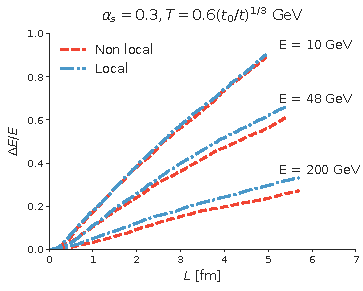
\includegraphics[width=\columnwidth]{Bjorken.pdf}
\caption{Energy loss fraction $\Delta E /E$ as function of path length $L$ at three different energies. Reddashed lines are direct simulations (the non-local case) and blue-dash-dotted lines are results using local approximation.}
\label{fig:Bjorken}
\end{figure}
Before applying the ``Modified rescattering" implementation to the heavy ion collisions, there are still a few issues to be studied and addressed.
The first one concerns with the coherence effect in an expanding medium. 
The QGP produced in colliders only exists for a short amount of time and it undergoes violent expansion, i.e, the medium temperature may have changed notably during the formation time.
Therefore, we expect different radiation spectrum and correspondingly different amount of energy loss between the following two computing scenarios:
\begin{itemize}
\item[1.]  {\it A non-local (direct) calculation}: radiated gluons can precept the changing medium within the formation times.
\item[2.] {\it A local approximation}: calculate with rates obtained in the infinite medium defined by the local temperature at the radiation vertex.
\end{itemize} 
Although a non-local scenario should be more realistic, we would like to see how close the local approximation is for a physical coupling $\alpha_s = 0.3$.
We set-up simulations in medium that undergoes Bjorken expansion at mid-rapidity \cite{PhysRevD.27.140}. 
The temperature decreases with proper time,
\begin{eqnarray}
T(\Delta\tau) = T_0 \left(\frac{\tau_0}{\tau_0+\Delta\tau}\right)^{\frac{1}{3}}.
\end{eqnarray}
We chose $T_0=0.6$ GeV, $\tau_0=0.6$ fm/c.
The ``Modified rescattering" approach is already a non-local calculation, because it preforms gluon rescatterings at different space-time during the evolution. 
To mimic the local approximation, we let each pre-gluon $i$ remember the temperature $T_i$ when it is first created and then perform rescatterings in an ``imaginary medium" defined by $T_i$.
The results are shown in Figure \ref{fig:Bjorken}. 
The difference between the two scenarios are negligible for $E=10$ GeV and is only moderate for a 200 GeV quark.
This is because for $\alpha_s = 0.3$, the ratio of the estimated maximum formation time $\sqrt{2x(1-x)E/\hat{q_0}}$ to the inverse temperature changing rate $(d\ln(T)/dt)^{-1}$,
\begin{eqnarray}
L_c \frac{d\ln(T)}{dt} = \sqrt{\frac{0.5 E}{6\pi C_A\alpha_s^2 T_0^3 9\tau\tau_0}} \approx \sqrt{\frac{0.7 \textrm{ fm/c}}{\tau_0+L}}
\end{eqnarray}
is not large after a few fermis. 
In more realistic event-by-event hydrodynamics simulations, the temperature profiles are much more complicated.
Initial condition fluctuations create medium hot spots and radial expansion boosts the fluid local  rest frame.
So it is still premature to conclude from this study in Bjorken flow that the local approximation is always justified.

\begin{figure}
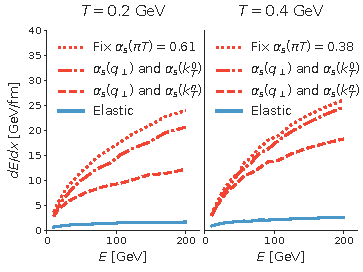
\includegraphics[width=\columnwidth]{Eloss_infinite_run.pdf}
\caption{Impact of the running coupling constant on the radiative energy loss. The dotted lines are calculated using fixed coupling $\alpha_s(2\pi T)$ for reference. The dashed-dotted lines uses the prescription $\alpha_s^{\textrm{el}}(q_\perp)$ and $\alpha_s^{\textrm{rad}}(k_{\perp,0})$. The dashed lines further modify the radiation vertex with $\alpha_s^{\textrm{rad}}(k_{\perp,n})$.}
\label{fig:run}
\end{figure}
Second, we improve the previous calculation with a running coupling constant, following the prescription described in \cite{Arnold:2008zu}.
This involves two changes in the formula. 
For elastic scattering vertices, $\alpha_s^{\textrm{el}}$ is evaluated at the $t$-channel momentum transfer squared. 
This is already the feature of {\tt Lido} with running coupling.
For splitting vertices,  $\alpha_s^{\textrm{rad}}$ should be evaluated at the final gluon transverse momenta squared,
\begin{eqnarray}\label{eq:kTn}
k_{\perp,n}^2 = \left(\vec{k}_T^0+\vec{q}_1+\cdots+\vec{q}_n\right)^2.
\end{eqnarray} 
In the {\tt Lido} model, the original scale used for $\alpha_s^{\textrm{rad}}$ is $k_{\perp,0}^2$ of the $2\rightarrow 3$ process.
Therefore, we modify the acceptance probability $p$ for the running coupling version from the one in Step 3.2 to
\begin{eqnarray}
p' = \min\left\{1, u\frac{\tilde{\lambda}}{\tau_f}\frac{\alpha_s(k_{\perp,n})}{\alpha_s(k_{\perp,0})}\right\}.
\end{eqnarray}
The order of magnitude of $k_{\perp,n}^2$ is $\sqrt{\hat{q}\omega}$ and it is about $\sqrt{\omega/T}$ times larger than $k_{\perp,0}^2$ for gluons in the LPM region, therefore the running coupling effect suppress the spectrum by another factor of $\alpha_s(k_{\perp,n})/\alpha_s(k_{\perp,0})$.
In Figure. \ref{fig:run}, we showed three calculations in a static medium. The dotted lines, as references, use a fixed coupling constant evaluated at a thermal scale $\alpha_s = \alpha_s(2\pi T)$ .
This scale is also the lowest scale cut-off for the running coupling constant in our model (note that this minimum scale is not required in the original work \cite{Arnold:2008zu}).
The dash-dotted lines are running coupling calculations where the $\alpha_s^{\textrm{el}}$ is evaluated at $\hat{t}$ and the $\alpha_s^{\textrm{rad}}$ at $k_{T,0}$.
The dashed lines are also running coupling calculations but evaluate $\alpha_s^{\textrm{rad}}$ at $k_{\perp,n}$ through the modified acceptance $p'$.
The running coupling effect results in a reduction of the energy loss compared to the fixed coupling references.

\begin{figure}
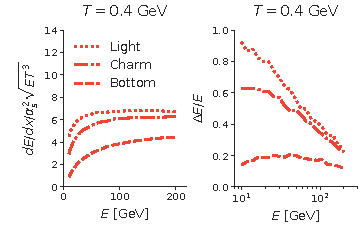
\includegraphics[width=\columnwidth]{Eloss_mass.pdf}
\caption{A demonstration of mass effect with $\alpha_s=0.3$, . Left plot: the scaled energy loss rate in an infinite medium for light quark, charm quark and bottom quark. Right plot: energy loss fraction of light quark, charm quark and bottom quark at path length $L=4$ fm.  }
\label{fig:mass}
\end{figure}

Finally, we put back the mass effects to treat the heavy quarks. These include the massive particle kinematics, a substitution in the formation time,
\begin{eqnarray}
(1-x)m_g^2 \rightarrow x^2M^2 + (1-x)m_g^2
\end{eqnarray}
and the so-called ``dead-cone" effect that suppresses collinear radiations with angles $\theta \sim k_\perp/k < M/E$. 
The massive version of the $2\rightarrow3$ improved Gunion-Bertsch matrix-element has been derived in \cite{Uphoff:2014hza}; however, since rescatterings increase the average $k_{\perp}^2$, a direct use of the massive $2\rightarrow3$ matrix-element in the ``Modified rescattering" approach leads to an unduly strong ``dead-cone" effect.
The solution is to use the $2\rightarrow3$ matrix-element without mass effect to generate initial gluons, while implementing the dead-cone suppression in another factor of the gluon acceptance probability,
\begin{eqnarray}
p'' = \min\left\{1, u\frac{\tilde{\lambda}}{\tau_f'}\frac{\alpha_s(k_{\perp,n})}{\alpha_s(k_{\perp,0})} \left[\frac{k_{\perp,n}^2}{k_{\perp,n}^2+x^2 M^2}\right]^4\right\}.
\end{eqnarray}
On the left of Figure \ref{fig:mass}, the scaled energy loss rate in an infinite medium is extracted from simulations for light (massless), charm ($M=1.3$ GeV) and bottom ($M=4.2$ GeV) quarks. 
On the right, it is the energy loss fraction at a finite path-length $L=5$ fm.
In both cases, the mass introduces the energy loss ordering, $\Delta E_{\textrm{light}} > \Delta E_c > \Delta E_b$ and the differences decrease at higher energy.

\begin{figure*}
\includegraphics[width=\textwidth]{raa_mclpm.pdf}
\caption{This figure shows what is predicted for D-meson observables at the leading order level considering running coupling and mass effect. The only parameter is the minimum scale in the running $\alpha_s(\max\{Q,\mu\})$. The solid lines use $\mu = 2\pi T$ and the dashed lines use $\mu=\pi T$}
\end{figure*}


\section{Summary and outlook}\label{section:summary}
To reduce the theory uncertainty introduced in the numerical implementation of the perturbative QCD transport of hard partons inside a quark-gluon plasma, we studied three different Monte-Carlo implementations and compare them to theory calculations.
We showed that the ``Modified rescattering" approach reproduces the coupling constant, temperature, parton energy and path-length dependences of the theoretical formula in both infinite- and thin-medium limits.
It also agrees with the predicted gluon spectrum within controlled uncertainty.
The expanding medium effect and running coupling effect are studied. For the application to the heavy-flavor sector, a tentative dead-cone effect implementation is proposed.
This approach is not restricted to scattering rate based model. 
It also applies to models with a diffusion treatment of the elastic processes. 
For future studies, controlling the uncertainties between Monte-Carlo implementation and theory helps to perform a more unambiguous examination of theory assumptions and a more meaningful phenomenology extraction of jet, heavy quark transport properties in a model-to-data comparison.
Moreover, a Monte-Carlo generator that is tuned to match leading order theory calculation could be a good starting point to implement next-to-leading-order effects in the phenomenology model.


\begin{acknowledgments}
SAB and WK are supported by the U.S. Department of Energy Grant no. DE-FG02-05ER41367. WK is also supported by NSF grant OAC-1550225.
\end{acknowledgments}

\begin{appendices}
\begin{figure}
\includegraphics[width=\columnwidth]{spectrum_E_alphas0d1.pdf}
\caption{The ratios of Monte-Carlo simulated spectra to the AMY NLL spectra (gray bands) and to the Gunion-Bertsch incoherent spectra (blue lines) are plotted, using $\alpha_s = 0.1$. The quark energy $E$ is 10, 50, 100, and 500 GeV as indicated by the rightmost vertical dashed lines in each subplot. The horizontal dashed lines denote $\pm 20\%$ deviation from unity.}
\label{fig:spectra-alphas=0.1}
\end{figure}

\begin{figure}
\includegraphics[width=\columnwidth]{spectrum_E_alphas0d3.pdf}
\caption{The same as Figure \ref{fig:spectra-alphas=0.1}, but for $\alpha_s = 0.3$.}
\label{fig:spectra-alphas=0.3}
\end{figure}
\end{appendices}
\section{The Gunion-Bertsch rate under soft transverse momenta exchange.}
\label{app:consistency}
The Gunion-Bertsch matrix-element factorizes the $2\rightarrow3$ process into the product of a $2\rightarrow2$ process and the radiative $1\rightarrow 2$ process. 
In the vacuum, this is,
\begin{eqnarray}
|M_{\textrm{GB}}|^2 &=& |M_{2\rightarrow 2}|^2 16 C_A \pi \alpha_s \frac{(1-\bar{x})^2q_\perp^2}{k_\perp^2\left(\vec{q}_\perp-\vec{k}_\perp\right)^2}.
\end{eqnarray}
In medium, a gluon thermal mass is used to regulate the divergence. 
For relatively hard splitting where $k_\perp \gg q_\perp \sim m_D$, 
\begin{eqnarray}
|M_{\textrm{GB}}|^2 &\approx & q_\perp^2 |M_{2\rightarrow 2}|^2 16 C_A \pi \alpha_s \frac{(1-\bar{x})^2}{k_\perp^4}.
\end{eqnarray}
Using this approximated from of $|M_{\textrm{GB}}|^2$ in the scattering rate Equation \ref{eq:GB-rate} and factorize the integration involving $q_\perp$ and $k_\perp$,
\begin{eqnarray}
\Gamma &=& \frac{1}{2E_1}\int\frac{f_i(p_2)d\vec{p_2}^3}{(2\pi)^3 2p_2}2\hat{s}\int d\hat{t}\frac{d\sigma_{2\rightarrow 2}}{d\hat{t}}q_\perp^2
\nonumber \\
&\times& \int 16\pi C_A \alpha_s \frac{(1-\bar{x})^2}{k_\perp^4} \frac{d\vec{k}^3}{(2\pi)^3 2k}
\end{eqnarray}
For the case of a quark, the first integration over the $2\rightarrow 2$ cross-section gives $C_F/C_A\hat{q}_g$, after summing over degeneracy of the gluonic and the fermionic scattering centers.
Then rewriting the second $k$ integration in terms of $x, k_\perp^2$ in the limit $\bar{x}\ll 1$, the rate becomes,
\begin{eqnarray}\label{eq:GB-LGV}
\Gamma &=& \hat{q}_g \int \frac{2C_F\alpha_s}{2\pi} \frac{dk_\perp^2}{k_\perp^4} \frac{dx}{x}
\end{eqnarray}
Finally, inserting the coherence factor of Equation \ref{eq:GB-rate-LPM}, the gluon radiation rate becomes identical to the one used in \cite{Cao:2013ita} when $x\ll 1$.
Reorganize the incoherent rate Equation \ref{eq:GB-LGV} perform the $k_\perp$ integration with the regulator $m_g$, we get,
\begin{eqnarray}
\Gamma &=& \int \frac{\alpha_s}{2\pi} \frac{2C_F}{x}dx \frac{q_g}{m_g^2} 
\end{eqnarray}
The factor $\frac{\hat{q}_g}{m_g^2}$ motivates our definition of the effective mean-free-path in Equation \ref{eq:effmpf}.

To estimate the order-of-magnitude of $\Delta t$ in the coherence factor, apply the condition \ref{eq:delta-t-1} and the above approximated formula,
\begin{eqnarray}
\nonumber
1 &\sim& \alpha_s\hat{q}\Delta t \int \frac{d\omega}{\omega}  \frac{dk_\perp^2}{k_\perp^4}  \left[1-\frac{\sin(\Delta t k_\perp^2/2\omega)}{\Delta t k_\perp^2/2\omega}\right]\\
\nonumber
&=& \alpha_s\hat{q}\Delta t^2 \int \frac{d\omega}{2\omega^2}  \int d\frac{2\omega}{\Delta t k_\perp^2}  \left[1-\frac{\sin(\Delta t k_\perp^2/2\omega)}{\Delta t k_\perp^2/2\omega}\right]\\
&=& \alpha_s\hat{q}\Delta t^3 \int \frac{d(\omega\Delta t)}{2(\omega\Delta t) ^2} f(2\omega\Delta t)
\end{eqnarray}
The limiting behavior of function $f(x)$ can be captured by a simple interpolation $Ax/(B+x)$, therefore the final integration only results in logarithmic dependence on the $\omega_{\min}\Delta t$ and $E\Delta t$.
So, the order of magnitude of a typical $\Delta t$ is $(\alpha_s\hat{q})^{-1/3}\sim 1/\alpha_s T$.


\section{Energy and coupling constant dependence of radiation spectra}\label{app:tune-spectrum}
It is important that we are aware of the known discrepancies between the Monte-Carlo implementation and the theory, particularly if one investigates an observable that is sensitive to the details of the spectra. 
In this appendix, we provide comparisons of radiation spectra at different energy and coupling constants for readers references.
Figure \ref{fig:spectra-alphas=0.1} and Figure \ref{fig:spectra-alphas=0.3} shows calculation using $\alpha_s = 0.1$ and $0.3$.
Within in each figure, different subplots vary the quark energy.
The gray bands are the ratios between the simulations and the AMY-NLL results (plotted for $\pi T < \omega < E$) and the blue lines are the ratios between the full simulations and the incoherent simulations (the Gunion-Bertsch rate, plotted for $0.1$ GeV $< \omega < 4\pi T $).
We notice that there are residue systematic logarithmic discrepancies from low energy to high energy.
The implementation also tends to generate less branching when $x \rightarrow 1$.

\bibliography{mclpm} 
\end{document}